\subsection{工具总体结构设计}
“四合一”通刮刷磁集成式井筒清洁工具\footnote{下文简称为“四合一工具”}是一种集机械刮削、刷洗清扫与强磁吸附功能于一体的井筒清洁装备。该工具主要用于清除套管内壁的水泥残留、铁屑、毛刺、石蜡及油污等沉积物，以满足新井射孔前的井筒净化要求，并为封隔器等密封工具提供合格的座封环境。同时，针对长期服役油井出现的套管内壁缩径、破裂及毛刺等损伤，该工具可辅助进行井筒内径检测与管壁修复。

工具的结构如图\ref{fig:structure_4_in_1}缩式，采用长轴式布局，主要由上接头、心轴系统、连接套、刮刀模块、毛刷模块、磁吸清理模块及辅助定位机构组成。各功能单元沿轴向依次排布，通过模块化连接方式实现组合，使工具兼具结构简洁性与操作灵活性。心轴作为核心承载部件，承担轴向推力、旋转载荷及各功能模块产生的反作用力，并确保各模块在工作过程中保持同轴状态。刮刀模块与毛刷模块可根据实际作业需求选装组合，以适应不同井况的清洁要求。

该工具的作业机制上是通过机械切削、挤压破碎与辅助清扫的协同作用实现套管内壁硬垢的高效清除。工作时，工具在外部驱动力作用下沿套管轴向运动，心轴将动力传递至各功能模块。刮刀模块中，安装于刀架上的齿形刮刀在弹簧预紧力作用下始终保持与管壁的贴合状态；当刀齿尖端接触硬垢层时，产生较大的局部接触应力，对垢层进行压入与剪切，促使硬垢内部萌生裂纹并逐步扩展，最终导致垢层破碎与剥离。采用弹簧浮动加载结构后，刀片可根据垢层厚度与管壁形态变化自动调节伸缩量，在维持稳定切削压力的同时避免刚性冲击对刀具造成的损伤。在刮削作业完成后，后方毛刷模块对破碎后残留的细小颗粒进行清扫，进一步提升管壁清洁度；磁吸模块则对清理过程中产生的铁磁性碎屑进行有效吸附，防止其再次沉积。此外，工具心轴上设置有扭曲弹簧部件，当刮刀遇到顽固坚硬杂物时可被压缩储能，通过障碍后释放能量以起到缓冲保护作用。通过刮削、刷洗与磁吸的多级协同，该工具能够实现对套管内壁硬垢的高效、彻底清除。

对应的工具规格分别为7\inch 、9-5/8\inch 和13-3/8\inch。提交了三种型号的工具设计图纸。


\begin{figure}[htbp]
	\centering
	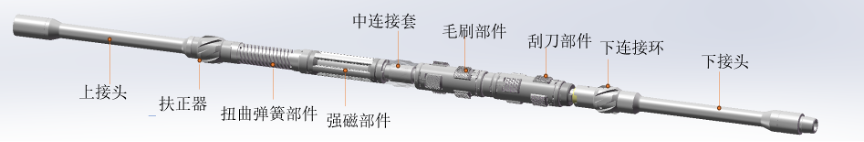
\includegraphics[width=1.\textwidth]{figure/chapter3/structure-4-in-1.png}
	\caption{四合一工具总体结构}
	\label{fig:structure_4_in_1}
\end{figure}

\begin{table}[htbp]
\centering
\caption{四合一工具技术参数}
\label{tab:zkg_params}
\begin{tabular}{cccccccccc} % 10列：型号、总长、水眼、套管磅级PPF、扶正体外径、刮刀外径范围、本体外径、接头扣、抗拉/抗扭强度
\toprule
规格 & \begin{tabular}[c]{@{}c@{}}总长\\ (mm)\end{tabular} & \begin{tabular}[c]{@{}c@{}}水眼\\ (mm)\end{tabular} & \begin{tabular}[c]{@{}c@{}}套管磅级\\ PPF\end{tabular} & \begin{tabular}[c]{@{}c@{}}扶正体\\ 外径\\ (mm)\end{tabular} & \begin{tabular}[c]{@{}c@{}}刮刀外径\\ (mm)\end{tabular} & \begin{tabular}[c]{@{}c@{}}本体外径\\ (mm)\end{tabular} & \begin{tabular}[c]{@{}c@{}}接头扣\\ (API)\end{tabular}& \begin{tabular}[c]{@{}c@{}}抗拉\\ (kN)\end{tabular} & \begin{tabular}[c]{@{}c@{}}抗扭\\（$\mathrm{kN\cdot m}$）\end{tabular} \\
\midrule
\multirow{4}{*}{7\inch} & \multirow{4}{*}{6500} & \multirow{4}{*}{40} & 17$\sim$20 & 158.24 & 159.77$\sim$171.96 & \multirow{4}{*}{139.7} & \multirow{4}{*}{NC38} & \multirow{4}{*}{1600} & \multirow{4}{*}{20} \\
& & & 20$\sim$26 & 155.58 & 155.70$\sim$167.89 & & & & \\
& & & 26$\sim$32 & 151.38 & 151.13$\sim$163.32 & & & & \\
& & & 32$\sim$35 & 146.05 & 146.56$\sim$158.75 & & & & \\
\midrule
\multirow{3}{*}{9-5/8\inch} & \multirow{3}{*}{6492} & \multirow{3}{*}{57.15} & 29.3$\sim$32.3 & 222.25 & 224.28$\sim$245.62 & \multirow{3}{*}{203.2} & \multirow{3}{*}{NC50} & \multirow{3}{*}{4000} & \multirow{3}{*}{50} \\
& & & 36$\sim$53.5 & 213 & 212.09$\sim$233.68 & & & & \\
& & & 47$\sim$59.4 & 209 & 209.04$\sim$230.38 & & & & \\
\midrule
\multirow{2}{*}{13-3/8\inch} & \multirow{2}{*}{6512} & \multirow{2}{*}{71.4} & 54.5$\sim$72 & 308 & 306.83$\sim$328.17 & \multirow{2}{*}{285.75} & \multirow{2}{*}{\begin{tabular}[c]{@{}c@{}}6-5/8\\ REG\end{tabular}} & \multirow{2}{*}{7800} & \multirow{2}{*}{110} \\
& & & 77$\sim$92 & 301.63 & 298.96$\sim$320.29 & & & & \\
\bottomrule
\end{tabular}
\end{table}

%对表中的数值进行说明：
%套管磅级：套管单位长度的重量，PPF：Pounds Per Foot（磅每英尺）

\subsubsection{四合一工具主要功能部件}

四合一工具主要功能部件如图\ref{fig:main_function_unite_4_in_1}所示。

刮刀模块（\ref{fig:mechanism_scratcher_4_in_1}）是工具完成硬垢破碎的核心部件，主要包括刀架、固定环、固定销、挡块、弹簧以及可更换齿形刀片。刀片安装于刀架槽内，在弹簧作用下能够产生径向浮动位移，使刀片能够适应套管内壁尺寸变化。当工具进入套管后，刀片受到管壁限制并保持与内壁接触。
        工具运动过程中，刀片齿尖首先接触硬垢层，通过较小接触面积形成较高局部压力，使垢层产生压裂和剪切破坏。当应力超过硬垢强度后，裂纹扩展并导致垢层剥离。
        
   毛刷模块(\ref{fig:mechanism_swiper_4_in_1})安装于刮刀模块后方，主要用于清除刮削后的残余垢屑。毛刷块同样采用浮动安装方式，可以根据套管内壁变化自动调整接触状态。在刮刀完成硬垢破碎后，毛刷通过柔性接触将附着的小颗粒和残余沉积物清除，提高最终清洁效果，降低碎屑重新附着的可能性。
   
   强磁部件（\ref{fig:mechanism_mag_sub_4_in_1}）通过固定销分别于两侧的挡环配合。主要作用是回收清洁过程中产生的磁性碎物。部分金属腐蚀产物和铁屑无法通过循环液及时排出，容易重新沉积于套管内部。强磁模块利用磁场吸附作用，将铁磁性颗粒吸附在工具表面，并随工具一起带出，实现井筒净化。
   
   扭曲弹簧（\ref{fig:mechanism_torsional_spring_4_in_1}）左端通过定位止转键，与左侧的扶正器的卡槽实现插接配合。右端以同样的方式与中挡环配合。工具中的扭曲弹簧部件不仅起到弹性支撑作用，还具有缓冲和保护功能。正常工作时，弹簧使刮刀片和毛刷块保持一定径向压力，保证其持续接触套管内壁。当遇到较坚硬或突出的杂物时，弹簧被压缩并储存能量，避免冲击载荷直接传递至工具连接部位；通过障碍后，弹簧释放能量，使刀片恢复工作位置，如图\ref{fig:flexible_scratch_system_4_in_1}所示。该结构提高了工具通过性和清洁稳定性，同时降低刀具损坏风险。
        
\begin{figure}[htbp]
    \centering
    % 子图 (a)
    \subfloat[刮刀部件结构]{%
        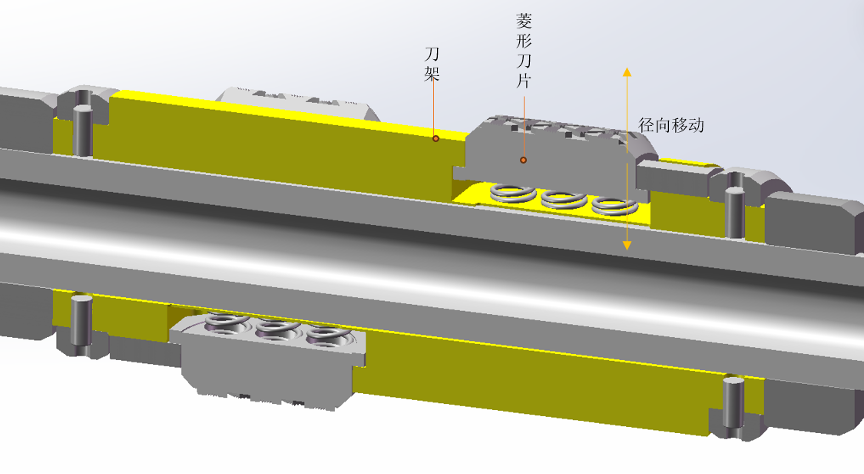
\includegraphics[width=0.45\linewidth]{figure/chapter3/mechanism-scratcher-4-in-1.png}%
        \label{fig:mechanism_scratcher_4_in_1}
    }
    \hfill
    % 子图 (b)
    \subfloat[毛刷部件结构]{%
        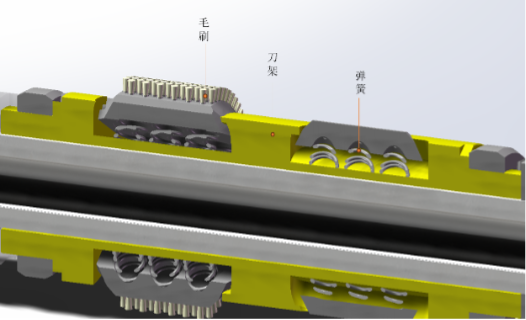
\includegraphics[width=0.45\linewidth]{figure/chapter3/mechanism-swiper-4-in-1.png}%
        \label{fig:mechanism_swiper_4_in_1}%
    }
    \vspace{1em}
      % 子图 (c)
    \subfloat[强磁部件结构]{%
        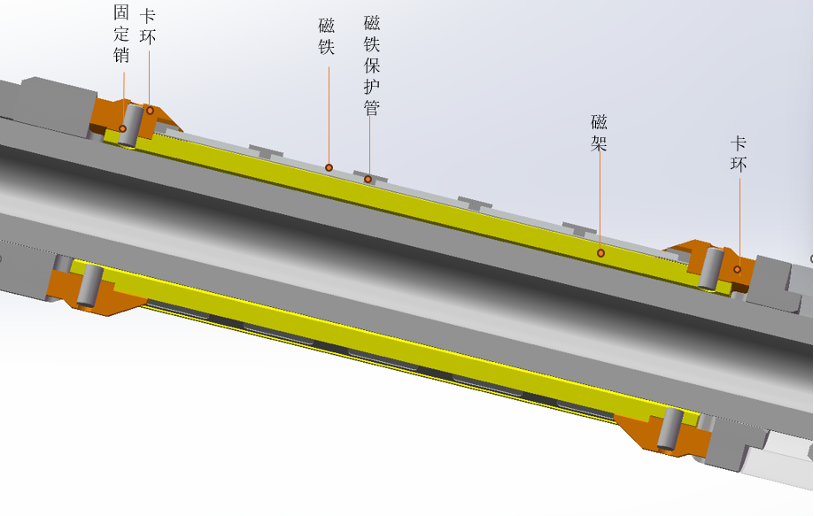
\includegraphics[width=0.45\linewidth]{figure/chapter3/mechanism-mag-sub-4-in-1.png}%
        \label{fig:mechanism_mag_sub_4_in_1}%
    }
    % 子图 (d)
    \subfloat[扭曲弹簧部件结构]{%
        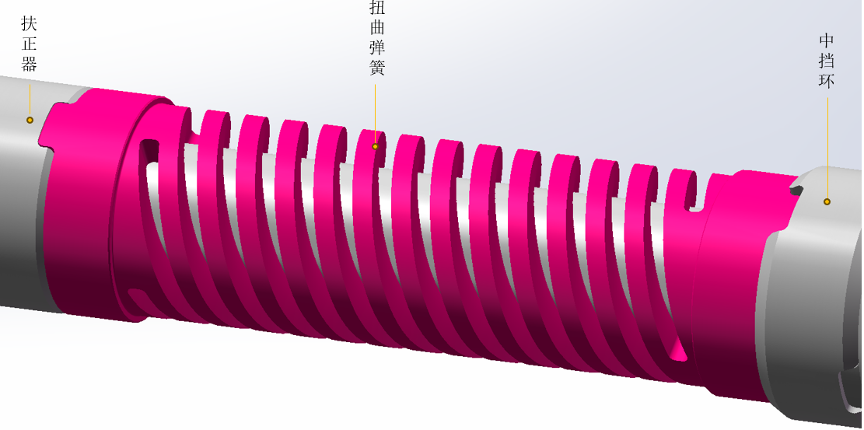
\includegraphics[width=0.45\linewidth]{figure/chapter3/mechanism-torsional-spring-4-in-1.png}%
      \label{fig:mechanism_torsional_spring_4_in_1}%
    }
    \caption{四合一工具主要功能单元}
        \label{fig:main_function_unite_4_in_1}
\end{figure}
      
\begin{figure}[htbp]
	\centering
	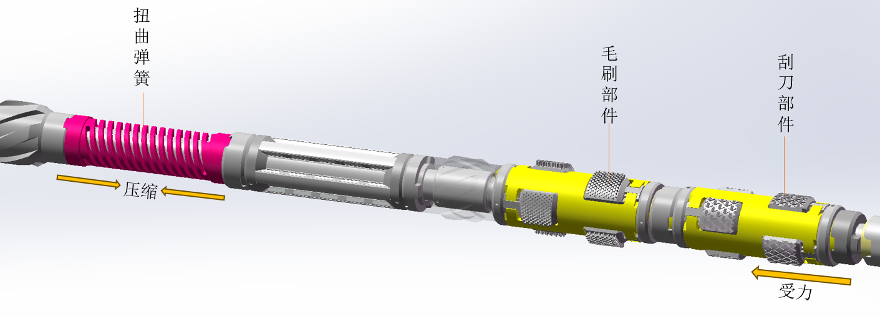
\includegraphics[width=.8\textwidth]{figure/chapter3/dynamic-system-torsional-spring-mechanism-4-in-1.png
}
	\caption{弹性刮削动力系统结构}
	\label{fig:flexible_scratch_system_4_in_1}
\end{figure}

\subsubsection{四合一工具辅助结构}

四合一工具辅助结构如图\ref{fig:additional_unite_4_in_1}所示。扶正器套装于心管外侧，轴向依靠上接头及下游组件的台阶端面限位，径向包覆螺纹连接部位。
扶正器外侧设计有螺旋导流槽，螺旋导流槽可以让钻井液/工作介质流过，不阻碍流体循环；支撑井壁使心管居中，承受径向摩擦载荷，保护心管与螺纹，改善工具下入性能。上接头作为四合一工具与外部管柱之间的连接部件，主要承担轴向载荷传递作用。其内部与心轴螺纹连接，使外部输入的轴向力能够有效传递至工具主体。
上接头外右侧空套一个扶正器。内六角凹端紧定螺钉使限制上接头与中心轴轴向移动，防止螺纹松动。

\begin{figure}[htbp]
    \centering
    % 子图 (a)
    \subfloat[上接头结构]{%
        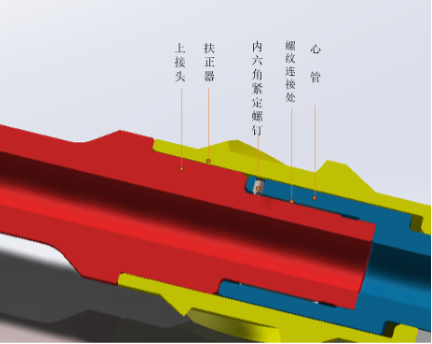
\includegraphics[width=0.4\linewidth]{figure/chapter3/upper-sub-4-in-1.png}%
        \label{fig:upper_sub_4_in_1}
    }
    %\hfill
    % 子图 (b)
    \subfloat[下接头结构]{%
        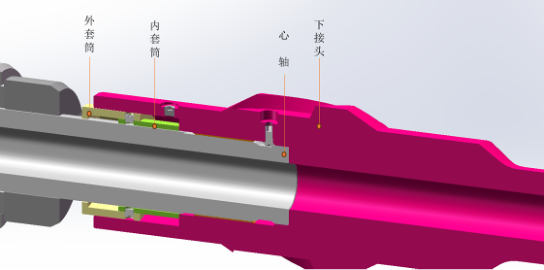
\includegraphics[width=0.5\linewidth]{figure/chapter3/lowwer-sub-4-in-1.png}%
        \label{fig:lowwer_sub_4_in_1}%
    }
    \caption{四合一工具辅助结构介绍}
        \label{fig:additional_unite_4_in_1}
\end{figure}

%\subsection{设计计算与校核}
\subsection[设计计算与校核]{设计计算与校核\protect\footnote{合同条款：5.2.1.3井筒高校清洁关键技术配套工具设计——（1）“四合一”集成式井筒清洁工具抗拉$>=100T$，抗扭$>17kN\cdot m$}}

%“2.75”-8 Stub ACME” 是一种常用于石油井下设备（如完井工具）的短牙梯形传动螺纹（Stub Acme Thread），ACME不是缩写，在机械工程领域，它特指 Acme Thread（爱克姆螺纹）。这是一种具有 29° 牙型角的梯形传动螺纹，其标准由美国标准协会（ANSI）制定。-8表示每英寸8个牙。
\subsubsection{主要受力件的螺纹强度校核}
四合一工具的主要受力件的螺纹强度危险点出现在心轴（图号：ZKG700004A）上，工具有三种规格，7\inch 规格的工具螺纹尺寸最小，最可能出现强度问题，于是螺纹抗拉强度校核以7\inch 规格作为计算依据，零件结构及尺寸如图\ref{fig:inner_pipe_for_strength_analysis}所示，其连接螺纹为2.75\inch -8 Stub ACME（爱克姆短牙梯形传动螺纹，8牙每英寸）。螺纹牙剪切强度计算：
\begin{equation}
\begin{aligned}
    F_{\max} &= [\tau] \cdot k_z \cdot \pi \cdot d_1 \cdot b \cdot z \cdot 10^{-3} \\
    [\tau] &= \frac{\sigma_s}{n}
\end{aligned}
\end{equation}
式中，$F_{\max}$---工具最大拉力，kN；

$[\tau]$---螺纹牙的剪切强度，MPa；

$k_z$---螺纹各圈的载荷不均系数，根据《机械设计手册》，取 $k_z = 0.56$；

$d_1$---螺纹底径，mm；

$b$---螺纹牙根宽度，mm；

$n$---安全系数，根据《机械设计手册》，取 $n = 2.5$；

$z$---旋合圈数；

$\sigma_s$---材料最小屈服强度，930 MPa (4330V-155 KSI)。
%4330V-155 KSI 是一种美标高强度低合金钢的牌号与强度等级组合标识，常用于石油、天然气及航空航天等对材料强度和韧性要求极高的领域。4330V：这是美国钢铁协会（AISI）标准下的合金结构钢牌号，属于镍铬钼钒系钢。它在4330钢的基础上添加了钒（V），以提升强度、硬度和抗疲劳性能。该材料通常经过真空电弧重熔（VAR）工艺处理，具有优异的淬透性、低温冲击韧性和抗裂纹扩展能力。155 KSI：表示该材料经热处理后达到的最小屈服强度为155千磅每平方英寸（KSI），换算约为1069 MPa。这属于超高强度级别，适用于承受极端载荷和冲击的工况。这种钢材的典型应用包括石油钻具、井下工具、航空紧固件和高应力传动部件。其化学成分中碳含量约0.28–0.33%，镍含量2.0–2.5%，铬0.6–0.9%，钼0.2–0.3%，钒0.15–0.3%，这些元素共同赋予其高强度与高韧性的平衡。

$2.75\inch - 8 \text{Stub ACME}$ 螺纹代入数据计算如下：
\begin{align*}
    F_{\max} &= [\tau] \cdot k_z \cdot \pi \cdot d_1 \cdot b \cdot z \cdot 10^{-3} \\
    &= 372 \times 0.56 \times 3.14 \times 67.94 \times 1.833 \times 35 \times 10^{-3} = 2851.13 \text{kN} \\
    &> 1000 \text{kN}
\end{align*}
于是，螺纹满足抗拉设计要求。

\begin{figure}[htbp]
	\centering
	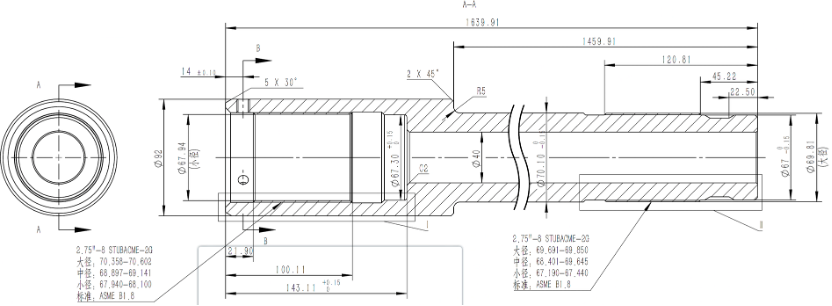
\includegraphics[width=1.\textwidth]{figure/chapter3/inner-pipe-for-strength-analysis.png}
	\caption{7\inch 规格工具的心轴结构}
	\label{fig:inner_pipe_for_strength_analysis}
\end{figure}

\subsubsection{主要受力件的零件强度校核}

清洁工具的主要受力件为芯轴危险截面有两处，分别为2.75”-8 Stub ACME外螺纹根部、2.75”-8 Stub ACME内螺纹根部。本文用解析法、数值模拟两种方法对心轴的强度进行校核。

（1）芯轴抗拉危险截面1：为2.75”-8 Stub ACME外螺纹根部。

对于环形零件截面，抗拉强度计算公式：
\begin{equation}
    F_{\max} = \frac{[\pi \cdot (D^2 - d^2)] \cdot \sigma_s}{4 \cdot n} \times 10^{-3}
    \label{eq:tensile_strength_circular_section}
\end{equation}
式中，$F_{\max}$——工具最大拉力，kN；

$D$——危险截面外径，mm；

$d$——危险截面内径，mm；

$\sigma_s$——材料最小屈服强度：930 MPa (4330V-155 KSI)；

$n$——安全系数，取 $n = 1.5$。

根据图\ref{fig:inner_pipe_for_strength_analysis}，取$D=67\textrm{mm}$，$d=40\textrm{mm}$，则心轴上$2.75\inch - 8 \cdot \text{Stub ACME}$ 外螺纹根部最大拉力：
\begin{align}
    F_{\max} &= \frac{\pi \cdot (D^2 - d^2) \cdot \sigma_s}{4 \cdot n} \times 10^{-3} \nonumber \\
    &= \frac{3.14 \times (67^2 - 40^2) \times 930}{4 \times 1.5} \times 10^{-3} \nonumber \\
    &= 1408.06 \, \text{kN} > 1000 \, \text{kN}
\end{align}

于是，危险截面1满足抗拉设计要求。

（2）心轴抗拉危险截面 2：为 $2.75\inch - 8 \text{Stub ACME}$ 内螺纹根部。

根据公式\ref{eq:tensile_strength_circular_section}和图\ref{fig:inner_pipe_for_strength_analysis}，取$D=92\textrm{mm}$。$d=71.6\textrm{mm}$（参见图纸ZKG700004A局部视图I），则心轴上$2.75\inch - 8 \text{Stub ACME}$ 外螺纹根部最大拉力：
\begin{align}
    F_{\max} &= \frac{[\pi \cdot (D^2 - d^2) ] \cdot \sigma_s}{4 \cdot n} \times 10^{-3} \nonumber \\
    &= \frac{[3.14 \times (92^2 - 71.6^2) ] \times 930}{4 \times 1.5} \times 10^{-3} \nonumber \\
    &= 1624.30 \, \text{kN} > 1000 \, \text{kN}
\end{align}

于是，危险截面2满足拉伸强度设计要求。


\subsubsection{主要受力件的零件强度抗扭校核}

四合一工具的受扭危险零件依然为\ref{fig:inner_pipe_for_strength_analysis}心轴螺纹结构根部截面，以及用于零件之间周向定位的端面键，如图\ref{fig:flat_shear_key}所示。下面进行螺纹危险截面的抗扭强度计算。截面抗扭强度$T_{\max}$计算式为
\begin{figure}[htbp]
	\centering
	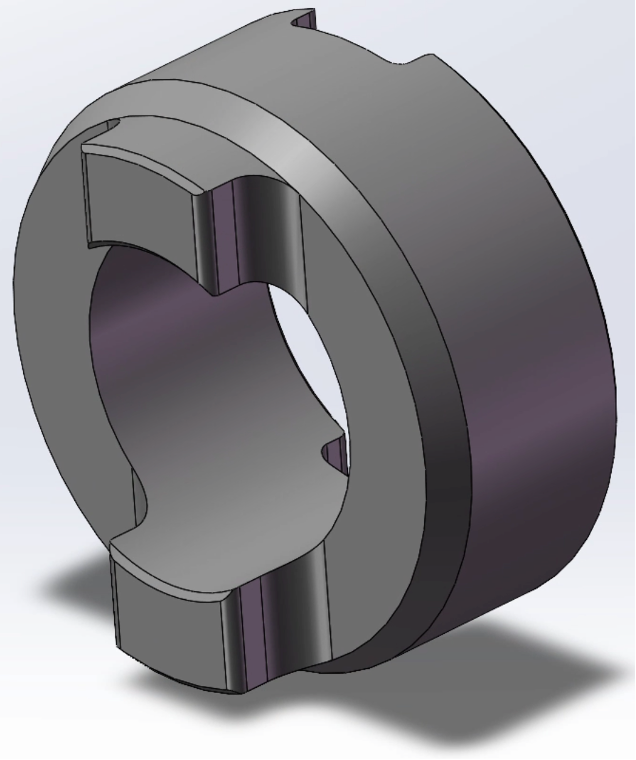
\includegraphics[width=.4\textwidth]{figure/chapter3/flat-shear-key.png}
	\caption{端面抗扭键结构}
	\label{fig:flat_shear_key}
\end{figure}

%\tau & =  \frac{16 \cdot D \cdot T_{\max}}{\pi \cdot (D^4 - d^4)} \times 10^6\\
\begin{equation}
\begin{aligned}	
    T_{\max} & =  \frac{[\tau] \cdot \pi \cdot (D^4 - d^4)}{16 \cdot D} \times 10^{-6}\\
    [\tau] &= n \cdot \sigma_s 
    \end{aligned}
\end{equation}
式中，$T_{\max}$——工具最大扭矩，kN·m；

$D$——危险截面外径，mm；

$d$——危险截面内径，mm；

$\sigma_s$——材料屈服应力，MPa；

$n$——安全系数，根据《机械设计手册》，取$n = 0.66$；

$[\tau]$——材料许用切应力，MPa。

对于心轴的危险截面1，代入材料的力学和几何参数计算得
\begin{align}
    T_{\max} &= \frac{[\tau] \cdot \pi \cdot (D^4 - d^4)}{16 \cdot D} \times 10^{-6} \nonumber \\
    &= \frac{613.8 \times 3.14 \times (67^4 - 40^4)}{16 \times 67} \times 10^{-6} \nonumber \\
    &= 31.63\,\text{kN} \cdot \text{m} > 17\,\text{kN} \cdot \text{m}
\end{align}

对于危险截面2，代入材料的力学和几何参数计算得
\begin{align}
    T_{\max} &= \frac{[\tau] \cdot \pi \cdot (D^4 - d^4)}{16 \cdot D} \times 10^{-6} \nonumber \\
    &= \frac{613.8 \times 3.14 \times (92^4 - 71.6^4)}{16 \times 92} \times 10^{-6} \nonumber \\
    &= 59.39\,\text{kN} \cdot \text{m} > 17\,\text{kN} \cdot \text{m}
\end{align}

于是，工具的两个危险截面都满足抗扭强度要求。

有限元计算结果如图所示。主要受力件为芯轴，危险截面出现在变径处，最大拉应力为1379MPa，最大剪切力为937MPa，建议在危险截面增加圆角以减小应力集中。

\begin{figure}[htbp]
	\centering
	\subfloat[拉伸载荷下应力分布]{%
	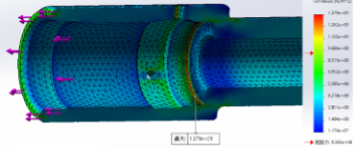
\includegraphics[width=0.7\textwidth]{figure/chapter3/inner-pipe-tensile-strength-simulation.png}
	}
	\vspace{1em}
	\subfloat[扭转载荷下应力分布]{%
	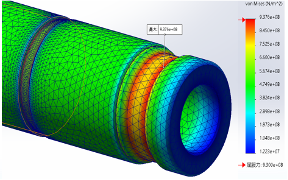
\includegraphics[width=0.7\textwidth]{figure/chapter3/inner-pipe-torsional-strength-simulation.png}
	}
	\caption{心轴零件受力有限元分析}
	\label{fig:FEA_verification_shaft}
\end{figure}

对于端面键，其材料牌号为4145H，抗扭危险截面为端面键截面（键的数量为 2）。

外筒件抗扭强度 $\tau$ 计算：
\begin{align}
    \tau &= \frac{T_{\max}}{b \cdot h \cdot d} \times 10^{-6} \\
    T_{\max} &= \frac{[\tau] \cdot b \cdot h \cdot d}{n_1} \times 10^{-6} \\
    [\tau] &= n \cdot \sigma_s = 0.66 \times 827\,\text{MPa} = 545.82\,\text{MPa}
\end{align}
式中，$T_{\max}$ —— 扭矩，$\text{kN}\cdot\text{m}$；

    $\sigma_s$ ——材料屈服应力，$\text{Mpa}$；
    
    $d$ ——危险截面内径，$\text{mm}$；
    
    $b$ ——端面键宽度，$\text{mm}$；
    
    $h$ ——端面键高度，$\text{mm}$；
    
    $n$ ——许用剪应力与许用拉应力系数，根据《机械设计手册》，取 $n=0.66$；
    
    $[\tau]$ ——材料许用切应力，$\text{Mpa}$；
    
    $n_1$ ——安全系数，取 $n_1=1.5$。

外筒件能承受的最大扭矩：
\begin{equation}
    T_{\max} = \frac{[\tau] \cdot b \cdot h \cdot d}{n_1} \times 10^{-6} = \frac{545.82 \times 30 \times 13.5 \times 90}{1.5} \times 10^{-6} = 13.29\,\text{kN}\cdot\text{m}
\end{equation}


\subsubsection{弹簧的力学计算}

四合一工具中设计了毛刷和刮板的预紧弹簧以及蓄能弹簧，如图\ref{fig:spring}所示。
\begin{figure}[htbp]
	\centering
	\subfloat[刮板、毛刷预紧弹簧]{%
	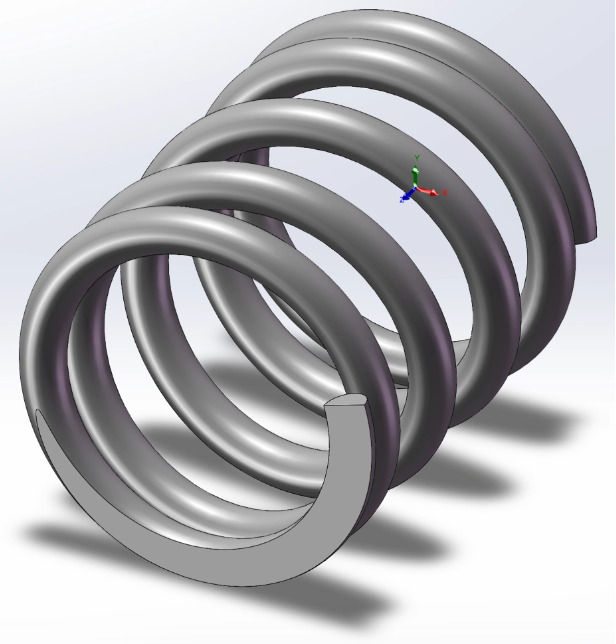
\includegraphics[width=0.2\textwidth]{figure/chapter3/pitch-spring.png}
	}
	%\vspace{1em}
	\subfloat[蓄能弹簧]{%
	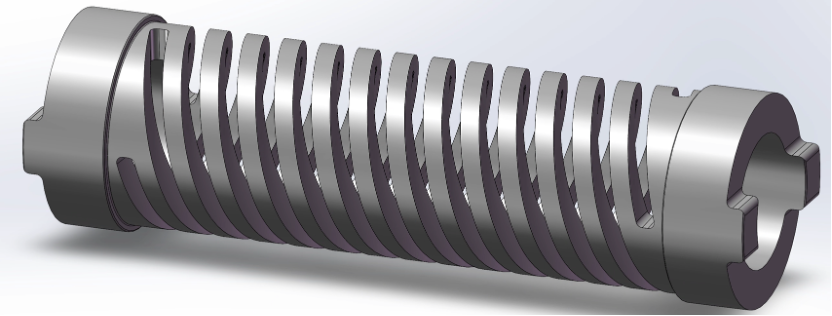
\includegraphics[width=0.55\textwidth]{figure/chapter3/oscillating-spring.png}
	}
	\caption{四合一工具中的弹簧零件}
	\label{fig:spring}
\end{figure}

毛刷和刮板的预紧弹簧参数列举于表\ref{tab:spring_parameters_pitch}，蓄能弹簧的参数列举于表\ref{tab:spring_params_rebounce}。
\begin{table}[htbp]
    \centering
    \caption{毛刷与刮板预紧弹簧技术参数表}
    \label{tab:spring_parameters_pitch}
    \renewcommand{\arraystretch}{1.3} % 增加行高，使表格更美观
    \begin{tabularx}{0.8\textwidth}{Xc}
        \toprule % 顶线
        \textbf{参数名称} & \textbf{数值} \\
        \midrule % 栏目线
        弹簧外径 $D$ & 25\,mm \\
        弹簧内径 $D_1$ & 19\,mm \\
        弹簧中径 $D_2$ & 22\,mm \\
        弹簧线径 $d$ & 3\,mm \\
        弹簧剪切弹性模量 $G$ & 79\,GPa \\
        弹簧自由高度 $H$ & 35\,mm \\
        弹簧总圈数 $n_1$ & 5 \\
        弹簧有效圈数 $n$ & 3 \\
        最小工作高度 $H_1$ & 29\,mm \\
        最大工作高度 $H_2$ & 23\,mm \\
        许用切应力 $[\tau]$ & 710\,MPa \\
        \bottomrule % 底线
    \end{tabularx}
\end{table}

\begin{table}[htbp]
    \centering
    \caption{弹簧技术参数表}
    \label{tab:spring_params_rebounce}
    \renewcommand{\arraystretch}{1.5} % 增加行高，使表格更美观
    \begin{tabularx}{0.8\textwidth}{Xc}  
        \toprule % 顶线
        \textbf{参数名称} & \textbf{数值} \\
        \midrule % 栏目线
        弹簧外径 $D$ & 120\,mm \\
        弹簧内径 $D_1$ & 80\,mm \\
        弹簧中径 $D_2$ & 100\,mm \\
        弹簧截面宽度 $b$ & 20\,mm \\
        弹簧截面高度 $h$ & 20\,mm \\
        弹簧剪切弹性模量 $G$ & 79\,GPa \\
        弹簧系数 $\gamma'$ & 5.57 \\
        弹簧系数 $\beta'$ & 2.404 \\
        弹簧自由高度 $H$ & 440\,mm \\
        弹簧总圈数 $n_1$ & 11 \\
        弹簧有效圈数 $n$ & 9 \\
        最小工作高度 $H_1$ & 400\,mm \\
        最大工作高度 $H_2$ & 390\,mm \\
        许用切应力 $[\tau]$ & 710\,MPa \\
        \bottomrule % 底线
    \end{tabularx}
\end{table}

刮刀与毛刷弹簧的力学计算如下。


弹簧刚度$P'$为
\begin{equation}
    P' = \frac{G \cdot d^4}{8 \cdot D_2^3 \cdot n} \times 10^{-3} = \frac{79000 \times 3^4}{8 \times 22^3 \times 3} \times 10^{-3} = 25 \, \text{N/mm}
\end{equation}

弹簧最小工作载荷$P_1$
\begin{equation}
    P_1 = P' \cdot (H - H_1) = 22 \times (35 - 29) = 132 \, \text{N}
\end{equation}

弹簧最大工作载荷$P_n$
\begin{equation}
    P_n = P' \cdot (H - H_2) = 22 \times (35 - 23) = 264 \, \text{N}
\end{equation}

弹簧旋绕比$C$
\begin{equation}
    C = \frac{D_2}{d} = \frac{22}{3} = 7.33
\end{equation}

弹簧曲度系数$K$
\begin{equation}
    K = \frac{4 \cdot C - 1}{4 \cdot C - 4} + \frac{0.615}{C} = \frac{4 \times 7.33 - 1}{4 \times 7.33 - 4} + \frac{0.615}{7.33} = 1.2
\end{equation}

弹簧最大切应力$\tau_{\max}$
\begin{equation}
    \tau_{\max} = \frac{8 \cdot K \cdot D_2}{\pi \cdot d^3} \times P_n = \frac{8 \times 1.2 \times 22}{3.14 \times 3^3} \times 264 = 657.7 \, \text{MPa} < 710 \, \text{MPa}
\end{equation}

于是，刮刀与毛刷强度满足要求。

蓄能弹簧的力学计算如下。

弹簧模块刚度$P'$
\begin{equation}
    P' = \frac{G \cdot b^2 \cdot h^2}{\gamma' \cdot D_2^3 \cdot n} = \frac{79000 \times 20^2 \times 20^2}{5.57 \times 100^3 \times 9} = 252 \, \text{N/mm}
\end{equation}

弹簧最小工作载荷$P_1$
\begin{equation}
    P_1 = P' \cdot (H - H_1) = 252 \times (440 - 400) = 10080 \, \text{N}
\end{equation}

弹簧最大工作载荷$P_n$
\begin{equation}
    P_n = P' \cdot (H - H_2) = 252 \times (440 - 390) = 12600 \, \text{N}
\end{equation}

弹簧旋绕比$C$
\begin{equation}
    C = \frac{D_2}{h} = \frac{100}{20} = 5
\end{equation}

弹簧曲度系数$K$
\begin{equation}
    K = \frac{4 \cdot C - 1}{4 \cdot C - 4} + \frac{0.615}{C} = \frac{4 \times 5 - 1}{4 \times 5 - 4} + \frac{0.615}{5} = 1.31
\end{equation}

弹簧最大切应力$\tau_{\max}$
\begin{equation}
    \tau_{\max} = \frac{\psi \cdot K \cdot D_2}{b \cdot h \cdot \sqrt{b \cdot h}} \cdot P_n = \frac{2.404 \times 1.31 \times 100}{20 \times 20 \times \sqrt{20 \times 20}} \times 12600 = 496 \, \text{MPa} < 710 \, \text{MPa}
\end{equation}

于是，蓄能弹簧的强度满足设计要求。



综合上述，各主要受力件的性能数据统计于表\ref{tab:force_data_statistics}中。


\begin{table}[htbp]
    \centering
    \caption{受力件数据统计表}
    \label{tab:force_data_statistics}
    \renewcommand{\arraystretch}{1.4} % 增加行高
    \begin{tabularx}{0.8\textwidth}{Xc}  % 关键：使用 tabularx + \textwidth + X列
        \toprule
        受力类型 & 数据\\
        \midrule
        NC38 最大拉力 & $3000\,\text{kN}$ \\
        材料屈服强度 $\sigma_s$ & $930\,\text{MPa}$ \\
        螺纹最大剪切力 $F_{\max1}$ & $2851.13\,\text{kN}$ \\
        芯轴最大拉力 $F_{\max2}$ & $1408.06\,\text{kN}$ \\
        NC38 最大扭矩 & $44.3\,\text{kN}\cdot\text{m}$ \\
        材料许用切应力 $[\tau]$ & $613.8\,\text{MPa}$ \\
        芯轴最大扭力 $T_{\max1}$ & $31.63\,\text{kN}\cdot\text{m}$ \\
        弹簧许用切应力 & $710\,\text{MPa}$ \\
        弹簧刚度 $P'$ & $22\,\text{N/mm}$ \\
        弹簧最小工作载荷 $P_1$ & $132\,\text{N}$ \\
        弹簧最大工作载荷 $P_n$ & $264\,\text{N}$ \\
        弹簧旋绕比 $C$ & $7.33$ \\
        弹簧曲度系数 $K$ & $1.2$ \\
        弹簧最大切应力 $\tau_{\max}$ & $657.7\,\text{MPa}$ \\
        外筒件抗扭 $T_{\max2}$ & $13.29\,\text{kN}\cdot\text{m}$ \\
        \bottomrule
    \end{tabularx}
\end{table}